\section*{SDR + MatLab}
\subsection*{Espectro en Análisis}
Utilizando el software MatLab, se realizó el análisis de la señal de radio FM en la frecuencia de $103.7MHz$. Se obtuvo la densidad espectral de potencia, el cual se muestra en la siguiente imagen.
\begin{figure}[H]
    \centering
    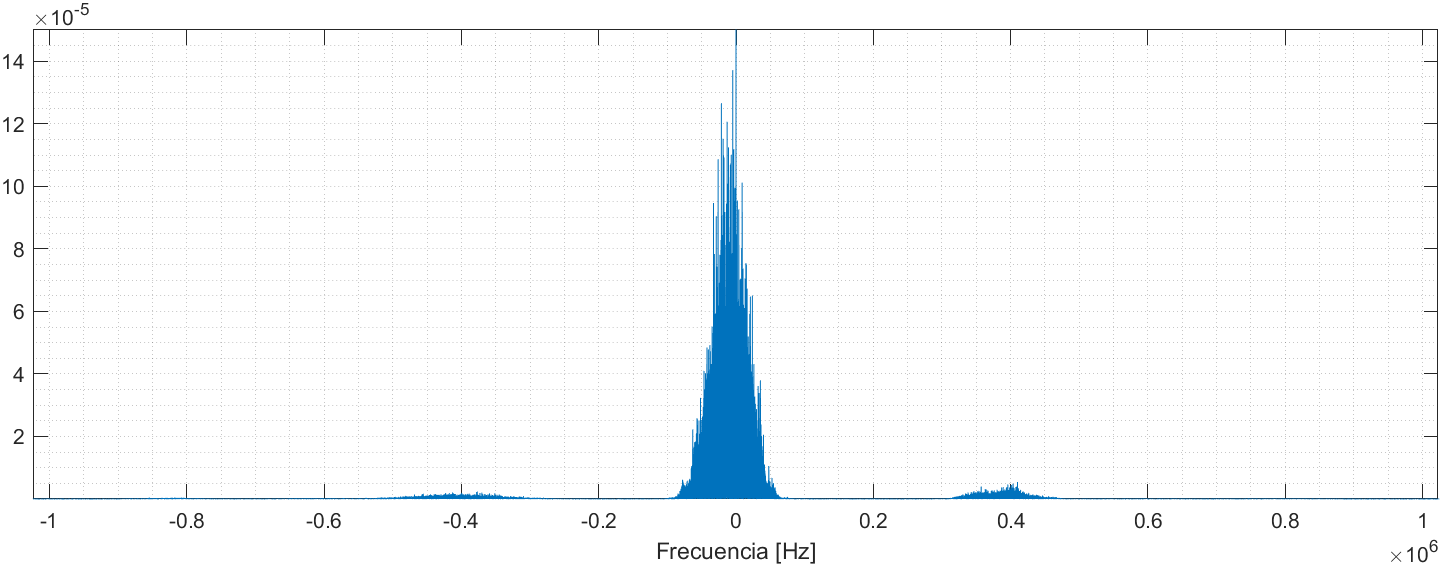
\includegraphics[width=\columnwidth]{images/2.1-original.png}
    \caption{Espectro de la señal de $103.7 MHz$}
    \label{fig:imagen4}
\end{figure}
En tal espectro se ve que existen componentes en la banda de los $264kHz$ pero se también se adiciona un espectro centrado en los $400kHz$ aproximadamente. Esto no corresponde a la estación buscada con lo cual utiliza un filtro butterworth de orden 5.
\begin{figure}[H]
    \centering
    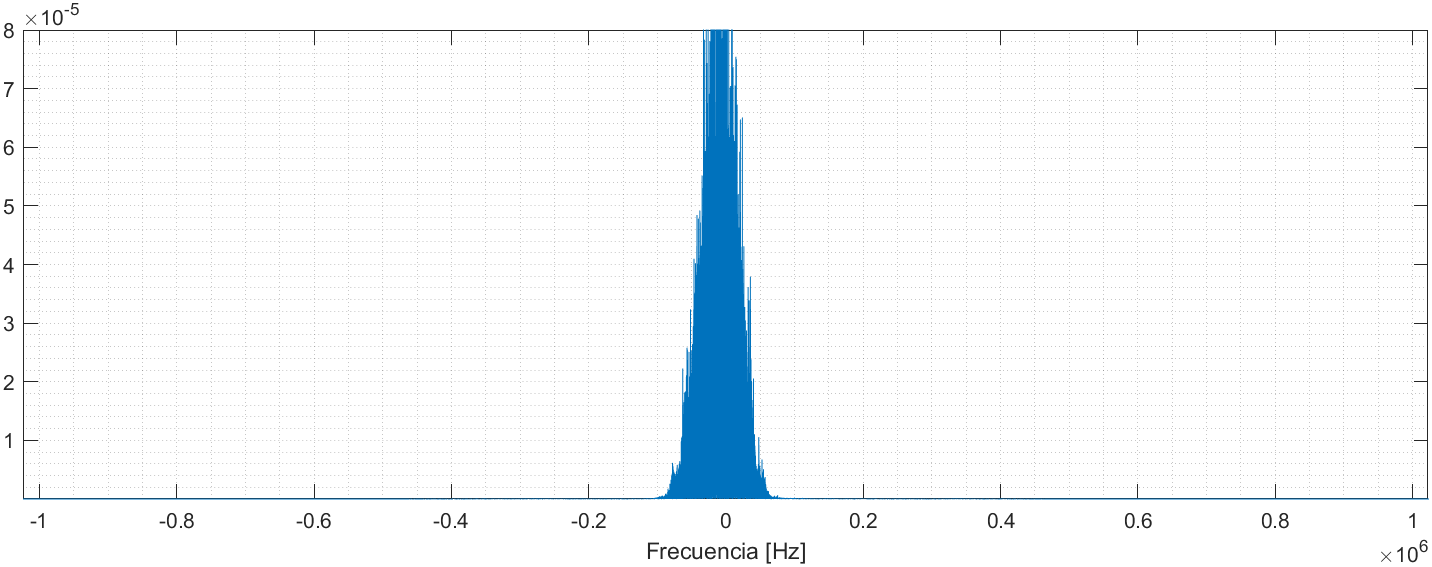
\includegraphics[width=\columnwidth]{images/2.2-filtrando.png}
    \caption{Espectro filtrado}
    \label{fig:imagen5}
\end{figure}
Una vez eliminado el espectro no deseado, se agrega un diezmado para que el procesamiento digital sea mas rápido al reducir la cantidad de muestras a procesar. Si se considera tener una señal que tenga un espectro de muestras entre $-120kHz$ y $120kHz$ cuando la frecuencia de muestreo era de $2048kHz$, se requiere:
$$
N_{1} = \frac{f_s}{2f_{lim}} = \frac{2048kHz}{2 \cdot 120kHz} = 8.53
$$
Utilizando $N_{1}=9$ se obtiene el espectro siguiente:
\begin{figure}[H]
    \centering
    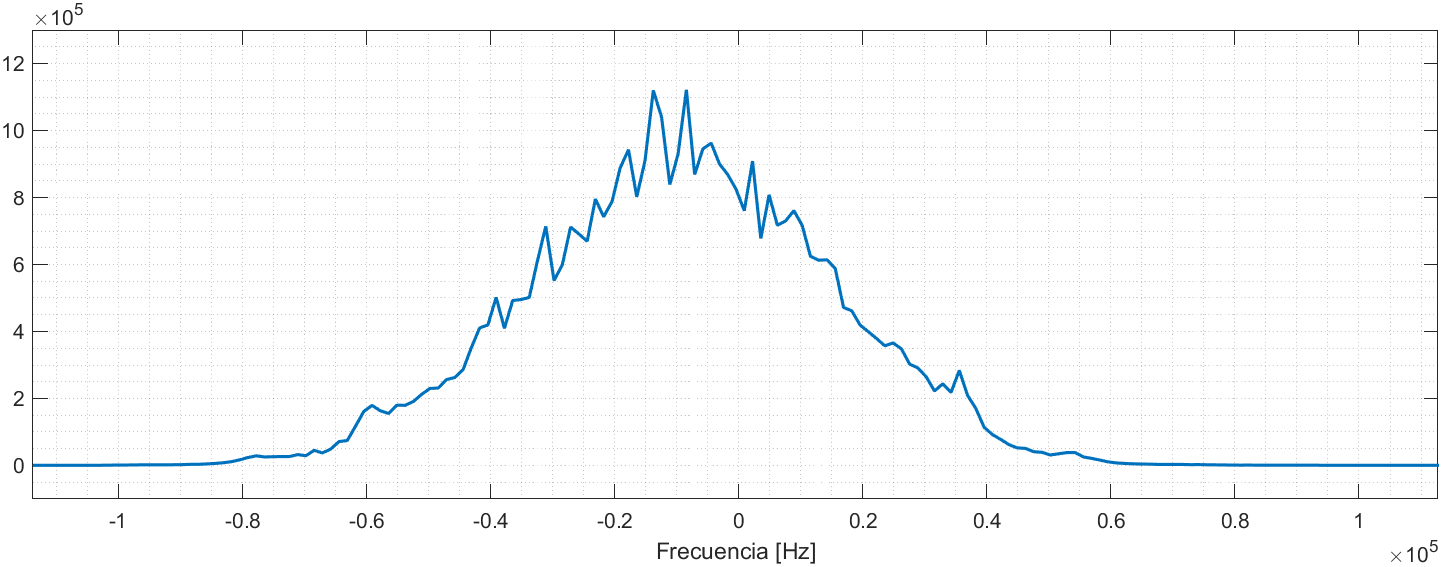
\includegraphics[width=\columnwidth]{images/2.3-diezmando.png}
    \caption{Espectro diezmado con $N_{1}=9$}
    \label{fig:imagen6}
\end{figure}
En este punto, ya se puede intentar obtener el mensaje \textit{MPX} descripto en la \hyperref[fig:imagen2]{Imagen 2}. Como el mensaje esta contenido en la fase de la señal, esto se modela como:
$$
f(t) = f_{c} + \underbrace{\dfrac{1}{2\pi} \dfrac{d\phi}{dt}}_{f_{d}}
$$
Entonces si:
$$
f_{d} = K_{f} \cdot m(t)
\hspace{2mm}\to\hspace{2mm}
m(t) = \dfrac{f_{d}}{2\pi K_{f}} \cdot \dfrac{d\phi}{dt}
$$
Como está definida la máxima desviación sobre la portadora siendo este valor de $75kHz$, se puede pensar que el mensaje entonces ya esta normalizado, dejando entonces $max\{m(t)\}=1$. En base a esto, la constante $K_{f}$ se puede calcular como:
$$
max\{f_{d}\} = K_{f} \cdot max\{m(t)\}
\hspace{2mm}\to\hspace{2mm}
K_{f} = 75kHz
$$
Ya teniendo este valor, solo resta usar la función \texttt{unwrap()} para eliminar los saltos de fase y luego aproximar la derivada con la función \texttt{diff()} junto a la frecuencia de muestreo para así obtener el mensaje MPX.
\begin{figure}[H]
    \centering
    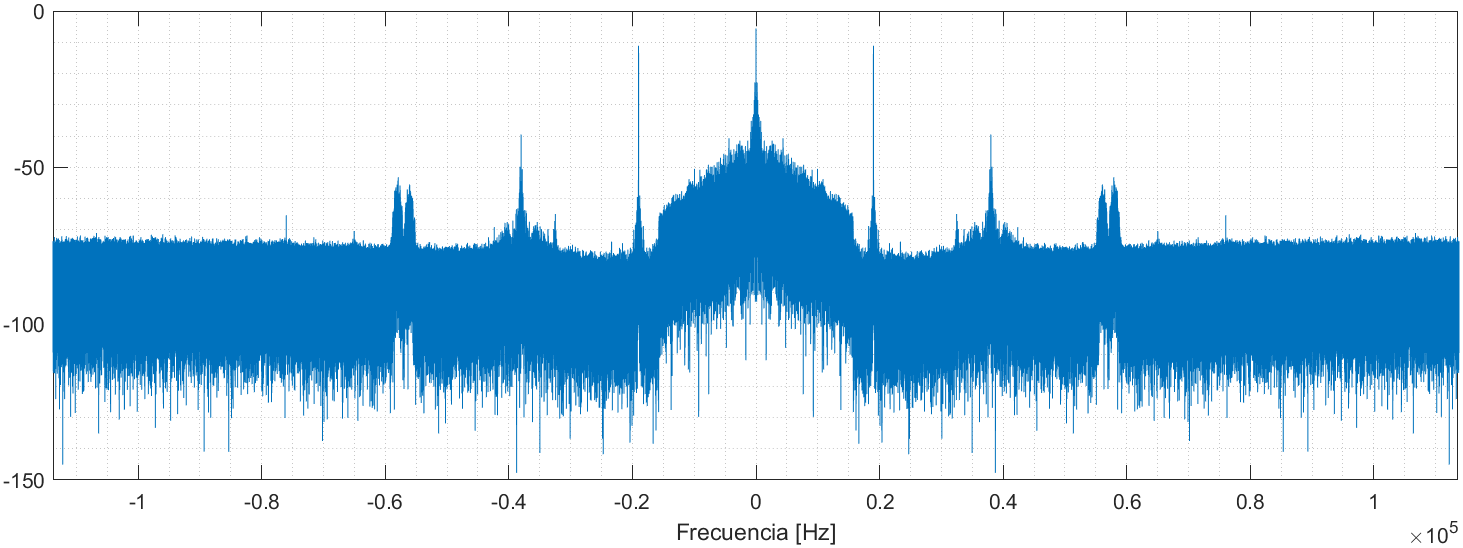
\includegraphics[width=\columnwidth]{images/2.4-mpx-completo.png}
    \caption{Espectro del mensaje MPX}
    \label{fig:imagen7}
\end{figure}
En esta ultima imagen, se puede observar que el mensaje $m(t)$ posee las características de la señal MPX, con una señal piloto de $19kHz$ y la señal de audio de $38kHz$. Finalmente, se ve en menor medida que existe espectro centrado en los $57kHz$ que corresponde a la señal de RDS.

Para obtener de forma sencilla el audio se utilizará unicamente la componente L+R, la cual es el espectro de la señal monoaural. Para esto se realiza un filtrado de la señal MPX en la banda de $0$ a $15kHz$ pero en este caso utilizando un filtro de orden $20$ para lograr mas selectividad ya que dejando el filtro de orden $5$ se requiere colocar la frecuencia de corte por debajo de los $8kHz$ atenuando la señal de audio que se quiere obtener.
\begin{figure}[H]
    \centering
    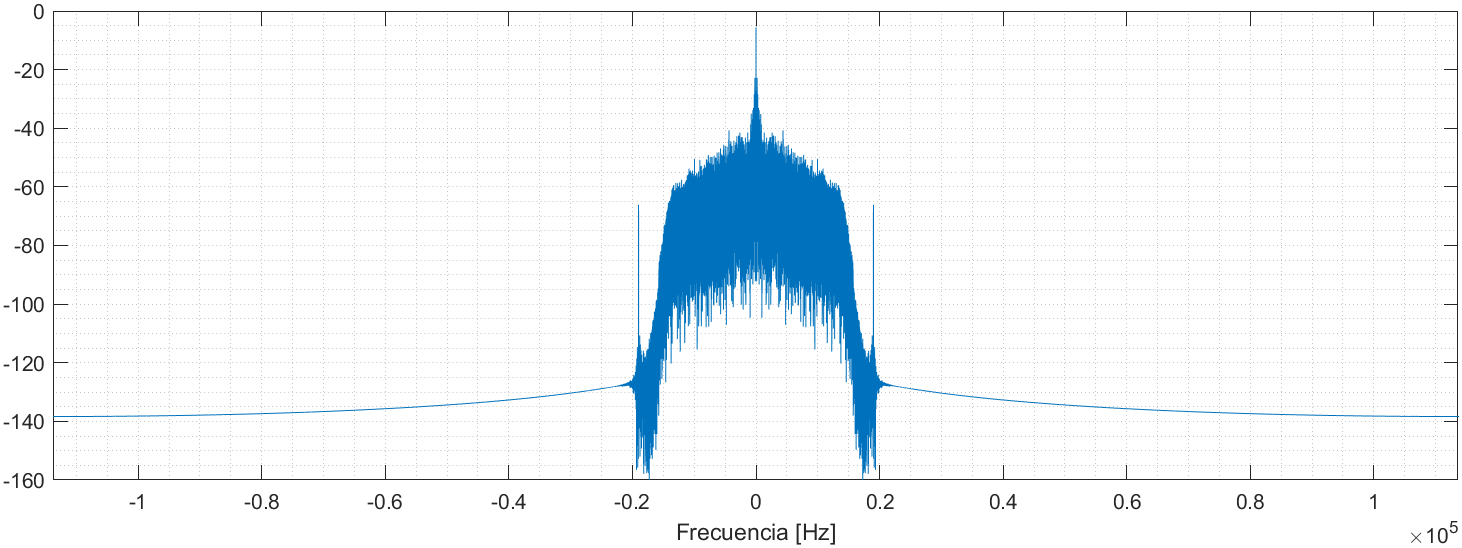
\includegraphics[width=\columnwidth]{images/2.5-mpx-filtrado.png}
    \caption{Espectro del mensaje MPX Filtrado}
    \label{fig:imagen8}
\end{figure}
Finalmente, se realiza un diezmado para lograr que la frecuencia de muestreo sea lo mas cercana a los $48kHz$, ya que en este punto, la $f^{*}_{s}=f_{s}/N_{1}$, entonces si busco los $48kHz$ requiero:
$$
f^{**}_{s} = \frac{f_{s}}{N_{1} N_{2}} = 48kHz
\hspace{2mm}\to\hspace{2mm}
N_{2} \approx 5
$$
Usando esto, la frecuencia de muestreo final sera de $f_{s} \approx 45kHz$ y graficando el espectro se puede ver:
\begin{figure}[H]
    \centering
    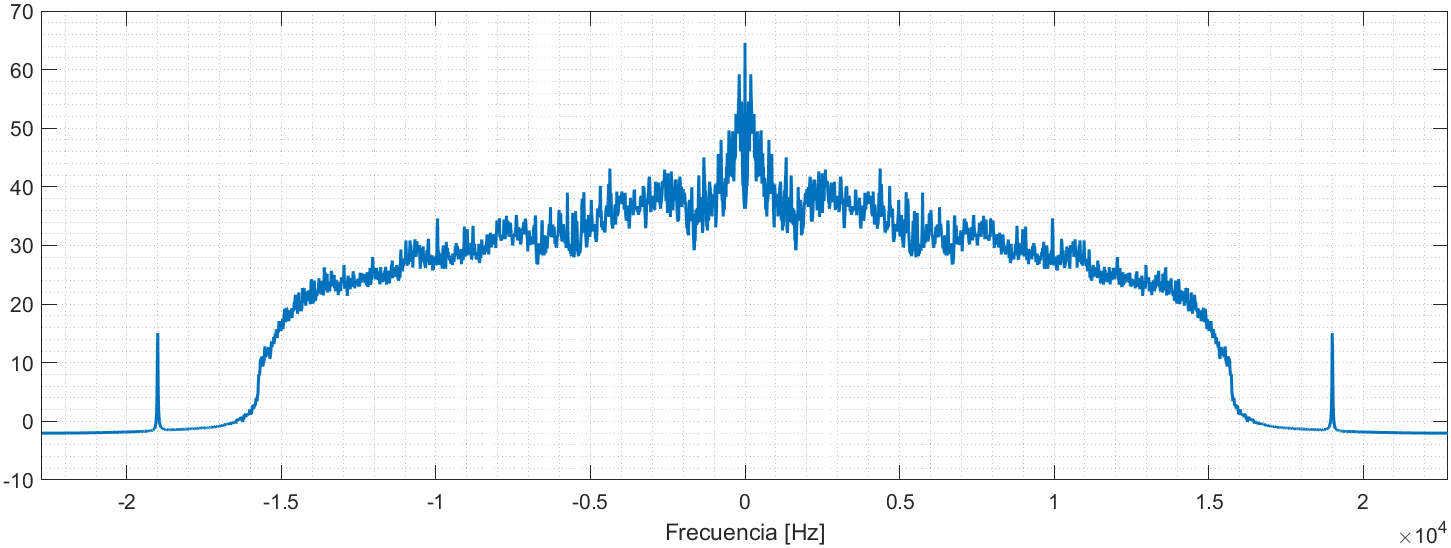
\includegraphics[width=\columnwidth]{images/2.6-mpx-final.png}
    \caption{Espectro audible (L+R)}
    \label{fig:imagen9}
\end{figure}
Finalmente, se puede escuchar el audio de la señal de radio FM en la frecuencia de $103.7 MHz$. Para esto se utilizó la función \texttt{soundsc()} de MatLab, la cual reproduce la señal de audio que es simplemente la salida del ultimo diezmador.



\hspace{1cm}